%!TEX root = thesis.tex

\chapter{Gesture recognition}
\label{ch:gestures}



\section{Feature extraction}



\subsection*{Segmentation - removing background}
\begin{figure}
        \center
        
\includegraphics[width=0.4\linewidth]{figures/pipeline/lefthand.jpg}
        \caption{Hand window }
        \label{fig:lefthandwindow}
\end{figure}
\begin{figure}
        \center
        
\includegraphics[width=0.4\linewidth]{figures/pipeline/lefthandcutout.jpg}
        \caption{Hand cutout }
        \label{fig:lefthandcutout}
\end{figure}
\begin{figure}
        \center
        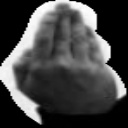
\includegraphics[width=0.4\linewidth]{figures/pipeline/lefthandhog.jpg}
        \caption{Hand features}
        \label{fig:lefthandfeatures}
\end{figure}

A cutout of a hand from a image still contains some background pixels, because a hand will never fill a perfect square. These pixels are unwanted since they contain arbitrary values that introduce noise into our process. In section \ref{sec:skinmodel} a binary mask for skin pixels is constructed. The binary inversion of this mask can be used again to remove the background. The result of this procedure can be seen in figure \ref{fig:gijs5_cutout}. To decrease the possibility that mislabeled skin pixels are removed by this mask, a small morphological dilate operation will increase the size of the hand cutout, but this will also introduce more noisy (background) pixels. 


\subsection*{Histogram of Oriented Gradients}
Histogram of oriented gradient (HOG) descriptors are feature descriptors used for object detection. It has been successfully applied and studied in human detection \cite{watanabe2009}.  The HOG descriptors method is similar to that of edge orientation histograms, scale-invariant feature transform descriptors, and shape contexts, but differs in that it uses a dense grid of uniformly spaced cells and uses overlapping local contrast normalization for improved accuracy.

For the experiments described in chapter \ref{ch:experiments} the same parameters as in the \cite{watanabe2009} paper are used, except that the image is not resized to 64 by 128 pixels, but 128 by 128 pixels.

hand detection with SIFT\cite{Wang_handposture}

\section{Classification}

\subsection*{Classifier}
KNN,  SVM

\subsection*{The stabilizer}
Thresholding histogram based stabilizer, maybe done before (better)?

\subsection*{Training phase}
recording video, manual labeling, extracting HOG features, training classifier

\section{Discussion}
